\section{Brass Soldering}

This section of the lab outlines the best practices and a standard operating procedure to join brass rods using lead solder.
%TODO: more

\subsection{Safety Precautions}

%TODO: List of equipment

The following safety precautions should be followed at all times.

\begin{enumerate}
\item Wear safety glasses when soldering and cutting rod.
\item Wear gloves while soldering.
\item Wash hands after soldering (Lead solder is used).
\item Use fume hood when soldering.
\item Ensure all equipment is powered off when not in use
\item Keep area around workstation clean of unnecessary tools and scrap material 
\end{enumerate}

\subsection{Standard Operating Procedure}

The following standard operating procedure was found to produce the best quality joints.

%TODO: More accurate based on what we discussed ?

\begin{enumerate}
\item Review safety precautions and ensure all guidelines are followed at each stage of the joining process.
\item Cut and grind the ends of the brass rods such that they contact fully for the desired angle for which they will be joined.
\item Place protective metal plate on table.
\item Clamp brass rods with joints to be soldered to the plate but ensure the joint is over the edge of the table in the desired position. Ensure the clamps are stiff and that the rods are unlikely to move during the soldering procedure.
\item Heat joint with soldering iron - apply only enough solder to the tip of the iron to ensure sufficient heat transfer to the joint.
\item Apply solder to joint, not to the tip of soldering iron.
\item Continue to heat the joint and apply solder until all sides are covered. 
\item Remove the soldering iron and solder and allow joint to cool.
\item Visually inspect and gently test joint by hand to ensure sufficient strength.
\item If the joint is critical and additional strength is required, solder a cross brace to the joint (see figure \ref{fig:solder_brace}).
\end{enumerate}

 \begin{figure*}[hp]
    \centering
    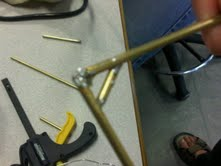
\includegraphics[width=0.6\textwidth]{images/solder_3}
    \caption{Joint Brace - Provides Significantly Improved Strength}
    \label{fig:solder_brace}
\end{figure*}

\subsection{Joint Analysis} 

Each joint created was qualitatively tested by hand until failure occurred.
Three important joint characteristics important to the final truss design were considered; flexibility, fragility, and failure mode.
Joints were found to have little flexibility.
Any bending observed was seen to occur in the brass members rather than the joint itself.
%	More of flexibility
Although it is difficult to state conclusively with so few samples, joints appeared to become more fragile after cyclic loading.
Joint strength was also seen to be highly dependent on the contact area between the solder and bras rods. 
Increasing the amount of solder generally increased strength.
The most likely failure mode was seen to be failure in bending. 
It was very difficult to pull the joints apart and cause then to fail by hand without bending them.
This was particularly true for joints with large amounts of solder.

\subsection{Conclusion}

From the first part of the lab, it is known the truss should not experience significant deformation. 
Since joints will be exposed to little bending and appeared quite strong in tension and compression, any well constructed joint is unlikely to fail.
Reinforcing joints with a cross member (as seen in figure \ref{fig:solder_brace}) added significant strength and should be done for critical joints.

